\documentclass{article}
\usepackage[utf8]{inputenc} %кодировка
\usepackage[T2A]{fontenc}
\usepackage[english,russian]{babel} %русификатор 
\usepackage{mathtools} %библиотека матеши
\usepackage[left=1cm,right=1cm,top=2cm,bottom=2cm,bindingoffset=0cm]{geometry} %изменение отступов на листе
\usepackage{amsmath}
\usepackage{graphicx} %библиотека для графики и картинок
\graphicspath{}
\DeclareGraphicsExtensions{.pdf,.png,.jpg}
\usepackage{subcaption}
\usepackage{pgfplots}
\usepackage{float}

\begin{document}
% НАЧАЛО ТИТУЛЬНОГО ЛИСТА
\begin{center}
    \Large
    Федеральное государственное автономное \\
    образовательное учреждение высшего образования \\ 
    «Научно-образовательная корпорация ИТМО»\\
    \vspace{0.5cm}
    \large
    Факультет программной инженерии и компьютерной техники \\
    Направление подготовки 09.03.04 Программная инженерия \\
    \vspace{1cm}
    \Large
    \textbf{Отчёт по лабораторной работе №2} \\
    По дисциплине «Методы оптимизации» (четвёртый семестр)\\
    \large
    \vspace{8cm}

    \begin{minipage}{.33\textwidth}
    \end{minipage}
    \hfill
    \begin{minipage}{.4\textwidth}
    
        \textbf{Студент}: \vspace{.1cm} \\
        \ Дениченко Александр P3212\\
        \textbf{Практик}:  \\
        \ Селина Елена Георгиевна
    \end{minipage}
    \vfill
Санкт-Петербург\\ 2024 г.
\end{center}
\pagestyle{empty}
% КОНЕЦ ТИТУЛЬНОГО ЛИСТА 
\newpage
\pagestyle{plain}
\section*{Данные}
Варинат 8
\[f(x) = \frac{x^7}{7} - x^3 + \frac{x^2}{2} - x\]
\[[a, b] = [1, 1.5]\]
\[\epsilon = 0.05\]
\section{Метод половинного деления}
Начальные значения границ:
\[[a, b] = [1, 1.5]\]
\begin{table}[ht]
    \centering
    \begin{tabular}{|c|c|c|c|c|c|c|c|}
        \hline
        Номер итерации & $a$    & $b$    & $x_1$    & $x_2$    & $f(x_1)$         & $f(x_2)$         & $b-a$   \\ \hline
        1              & 1.225  & 1.500  & 1.225    & 1.275    & -1.722           & -1.752           & 0.275   \\
        2              & 1.225  & 1.388  & 1.338    & 1.388    & -1.742           & -1.682           & 0.162   \\
        3              & 1.225  & 1.331  & 1.281    & 1.331    & -1.754           & -1.746           & 0.106   \\
        4              & 1.253  & 1.331  & 1.253    & 1.303    & -1.743           & -1.755           & 0.078   \\ \hline
        \end{tabular}
    \caption{Ручной подсчёт}
    \label{your-label}
\end{table}
Произошло выполнение предиката: 
\[b - a > 2\cdot \epsilon\]
Поэтому подсчитаем ответ: 
\[x = \frac{b+a}{2} = \frac{1.331+1.253}{2} = 1.292\]
\[y = f(x) = -1.756\]

\section{Метод золотого сечения}

Просчитаем первую итерацию: 
\[x_1 = a+0.382\cdot (b -a) =1.191;\ x_2 = a+0.618\cdot (b-a) = 1.309;\] 
\[f(x_1) = -1.686;\ f(x_2) = -1.754\]
Так как 
\[f(x_1) > \ f(x_2)\]
То оставляем интервал:
\[[x_1, b]\]
\[[1.191, 1.5]\]
На второй итерации $x_1$ полагаем равным $x_2$, который вычисляется по формуле 
\[x_2 = a + 0.618 \cdot (b - x_1) = 1.191 + 0.618\cdot (1.5 - 1.309) = 1.30903\]
Так же вычисляем зничение функции в точке $x_2$:
\[f(x_2) = -1.75443\]
Значение функции в $x_1$ уже было вычислено на предыдущем шаге.\\
Далее повторяем для 5 итераций и на каждой итерации проверяем: 
\[f(x_1)<f(x_2)\ =>\ [a, x_2];\ x_2 = x_1;\ x_1 = a+0.382(x_2-a)\]
\[f(x_1)\geq f(x_2)\ =>\ [x_1, b];\ x_1 = x_2;\ x_2 = a + 0.618 \cdot (b - x_1)\]
\begin{table}[H]
    \centering
    \begin{tabular}{|c|c|c|c|c|c|c|c|}
        \hline
        Iter. & $a$           & $b$               & $x_1$            & $x_2$            & $f(x_1)$                 & $f(x_2)$                 & $|b-a|$                  \\ \hline
        1     & 1.000         & 1.500             & 1.191            & 1.309            & -1.6855     & -1.75444     & 0.500                    \\
        2     & 1.191         & 1.500             & 1.309            & 1.30903 & -1.75444   & -1.75443     & 0.309                    \\
        3     & 1.191         & 1.30903 & 1.229704        & 1.309            & -1.72569      & -1.75444      & 0.118038      \\
        4     & 1.2297      & 1.30903 & 1.309            & 1.22972      & -1.75444      & -1.72571       & 0.07933     \\
        5     & 1.2297      & 1.22972        & 1.25571 & 1.309          & -1.74404      & -1.75444      & $2.3\cdot 10^{-5}$    \\ \hline
        \end{tabular}
    \caption{Ручной подсчёт}
    \label{tab:golden-section-search}
\end{table}
На 5 итерации получили абсолютную разницу границ интервала меньше чем заданная погрешность, тогда ответ:
\[x = \frac{a-b}{2} = \frac{1.22972 - 1.2297}{2} = 1.22971\]

\section{Метод хорд}
Для перовой итерации:
\[x = a - \frac{f'(a)}{f'(a)-f'(b)}(b-a) = 1 - \frac{-2}{-2-5.141}(1.5 -1) = 1.140 \]
\[|f'(1.140)| = 1.564\]
\[1.564 > \epsilon\ => \ \text{продолжаем цикл}\]
\begin{table}[H]
    \centering
    \begin{tabular}{|c|c|c|c|c|c|c|}
    \hline
    Итерация & $a$    & $b$  & $f'(a)$ & $f'(b)$ & $x$    & $|f'(x)|$ \\ \hline
    1     & 1.000  & 1.5  & -2.000  & 5.141   & 1.140  & 1.564     \\
    2     & 1.140  & 1.5  & -1.564  & 5.141   & 1.224  & 0.908     \\
    3     & 1.224  & 1.5  & -0.908  & 5.141   & 1.265  & 0.433     \\
    4     & 1.265  & 1.5  & -0.433  & 5.141   & 1.284  & 0.186     \\
    5     & 1.284  & 1.5  & -0.186  & 5.141   & 1.291  & 0.077     \\ \hline
    \end{tabular}
    \caption{Ручной подсчёт}
    \label{tab:newton-raphson-summary}
\end{table}
Пяти итераций недостаточно, но критерий для сравнения понижается на каждом шаге, что говорит о сходимости метода

\section{Метод Ньютона (касательных)}
Взяли начальное приближение $x_0 = 1.25$\\
Первая итерация:
\[F(1.250) = f'(1.250) = -0.623\]
\[F'(1.250) = f''(1.250) = 11.811\]
\[x_1 = x_0 - \frac{F(x_0)}{F'(x_0)} = 1.25 - \frac{-0.623}{11.811} = 1.303\]
\begin{table}[H]
    \centering
    \begin{tabular}{|c|c|c|c|c|c|}
    \hline
    Итерация & $x$     & $F(x)$  & $F'(x)$  & $x_k$  & $|f'(x)|$                 \\ \hline
    1        & 1.250   & -0.623   & 11.811    & 1.303    & 0.62            \\
    2        & 1.303   & 0.099    & 15.696    & 1.296    & 0.099       \\
    3        & 1.296   & 0.002    & 15.192    & 1.296    & 0.002        \\ \hline
    \end{tabular}
    \caption{Ручной подсчёт}
    \label{tab:optimization-method-summary}
\end{table}

Так как 
\[|f'(x_3)| = 0.002 < \epsilon\]
тогда ответ
\[x = 1.296; \ y = -1.756\]

\end{document}
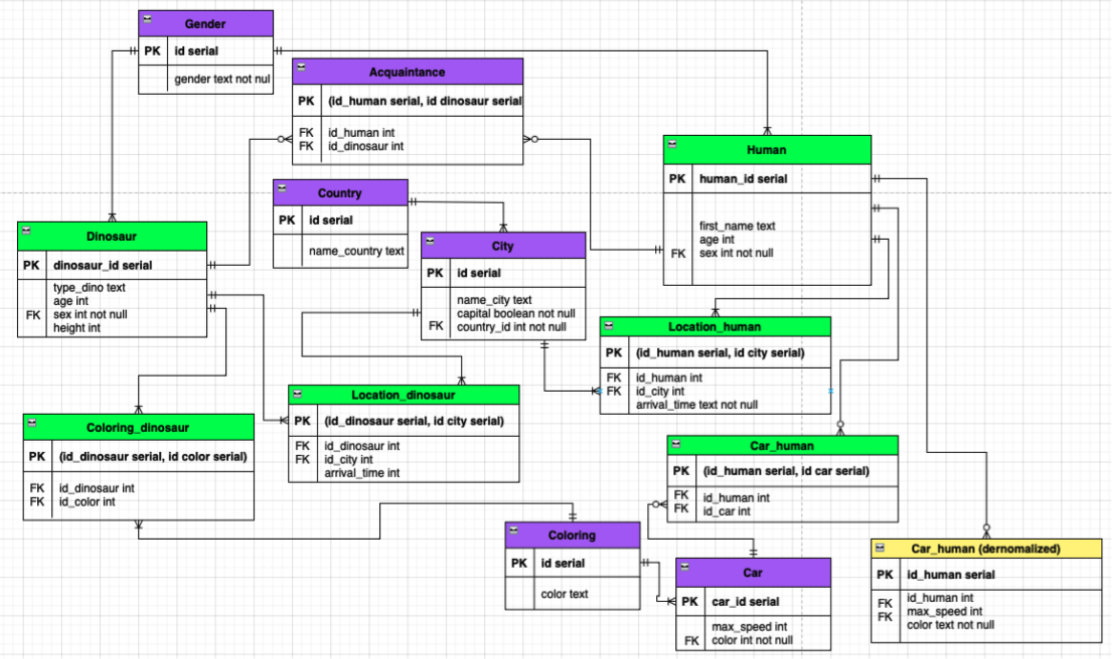
\includegraphics[width=.9\textwidth]{123}